\chapter{Creating and Running Instances}
\par In this section we will add User accounts in keystone who can use Openstack services.
%Intro\footnotemark\\
\begin{spacing}{1.2}
%note en bas de page
\section{Creating an authentication config file for our new user hiroshima}

\par We will connect with a user and create a configuration for the authentication of
Keystone. To do this, we will leave the root, then modify  / keystonerc and display the list
[flavor] available: 
\\
\begin{figure}[!htb] 
\begin{center} 
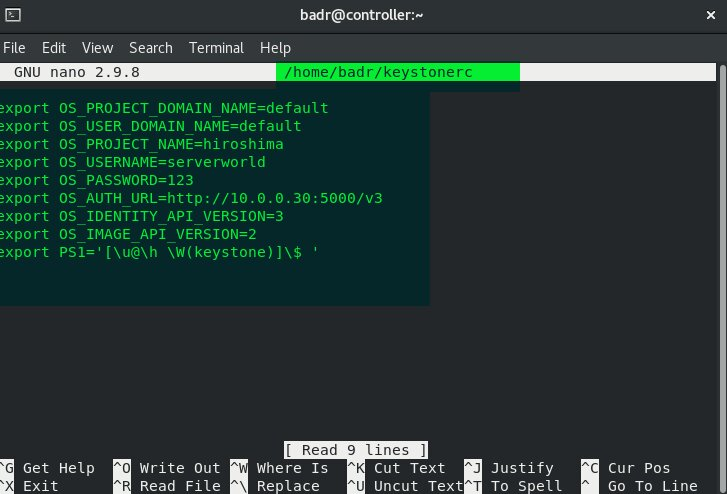
\includegraphics[width=1\linewidth]{Cloud/Creating and Running Instances/configuring environment variables} 
\end{center} 
\caption{configuring environment variables} 
\end{figure} 
\FloatBarrier
\\
\begin{figure}[!htb] 
\begin{center} 
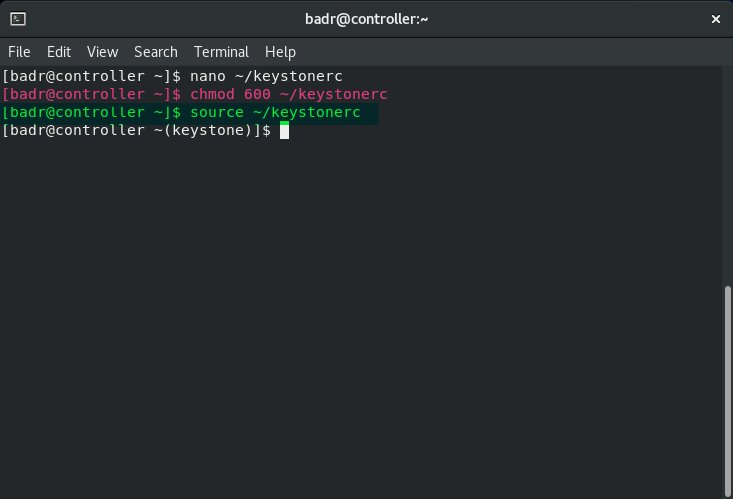
\includegraphics[width=1\linewidth]{Cloud/Creating and Running Instances/chmod and source} 
\end{center} 
\caption{using the freshly created config file in order to connect as hiroshima} 
\end{figure} 
\FloatBarrier
\\


\\
\par From now on, the commands we will be preforming in this section are perfomed as the user hiroshima.
\\
\par Let's display the list of available images: 
\\
\begin{figure}[!htb] 
\begin{center} 
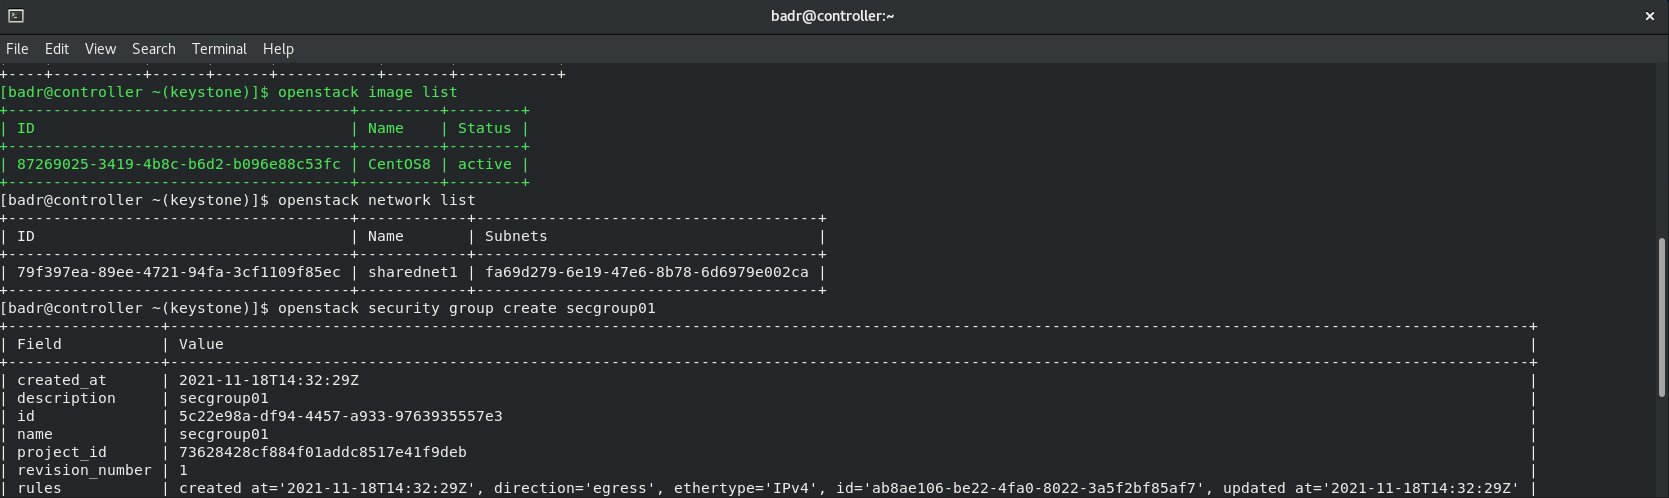
\includegraphics[width=1\linewidth]{Cloud/Creating and Running Instances/show available image list} 
\end{center} 
\caption{show available image list} 
\end{figure} 
\FloatBarrier

\par We will create a safety group for the instances:
\\
\begin{figure}[!htb] 
\begin{center} 
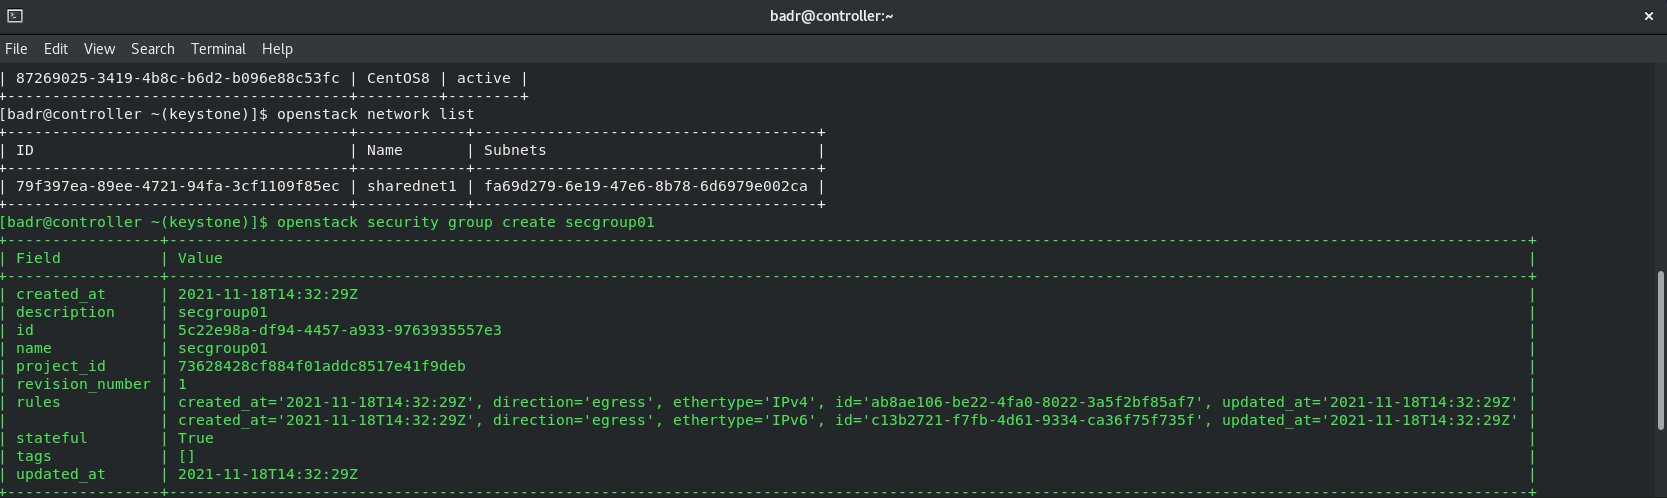
\includegraphics[width=1\linewidth]{Cloud/Creating and Running Instances/creating safety group} 
\end{center} 
\caption{creating safety group} 
\end{figure} 
\FloatBarrier

\\\par To verify this, we can display the list of security groups: 
\\
\begin{figure}[!htb] 
\begin{center} 
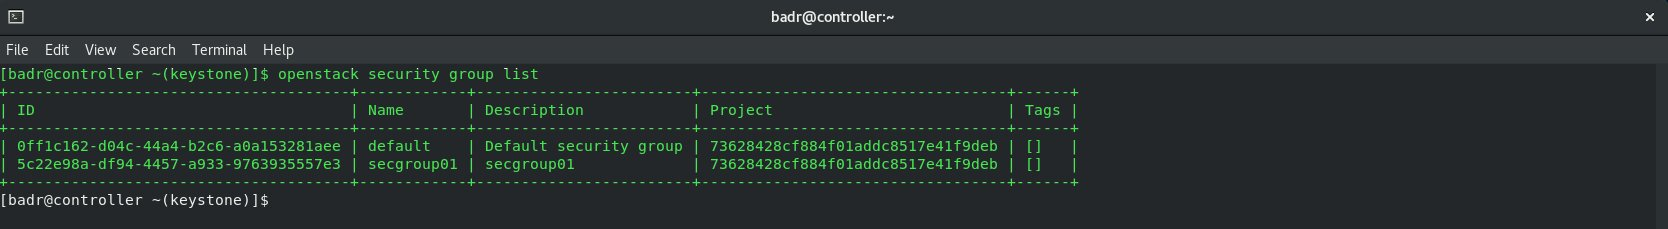
\includegraphics[width=1\linewidth]{Cloud/Creating and Running Instances/check security group} 
\end{center} 
\caption{check security group} 
\end{figure} 
\FloatBarrier
\\

\par Next, we will create an SSH key pair for connection to instances and add a key
public:
\\
\begin{figure}[!htb] 
\begin{center} 
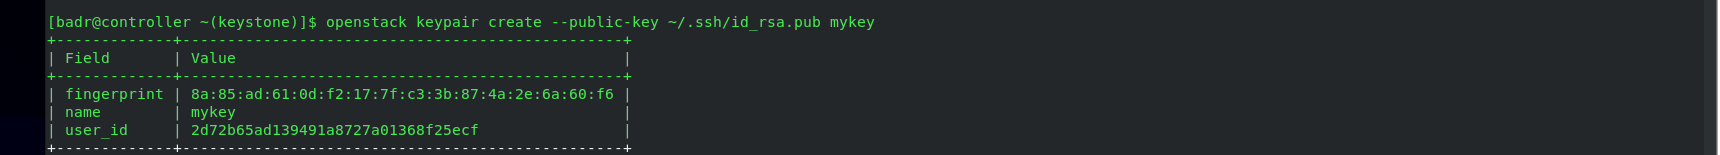
\includegraphics[width=1\linewidth]{Cloud/Creating and Running Instances/add public-key} 
\end{center} 
\caption{add public-key} 
\end{figure} 
\FloatBarrier
\\
\par We are ready to create and start an instance: 
\\
\begin{figure}[!htb] 
\begin{center} 
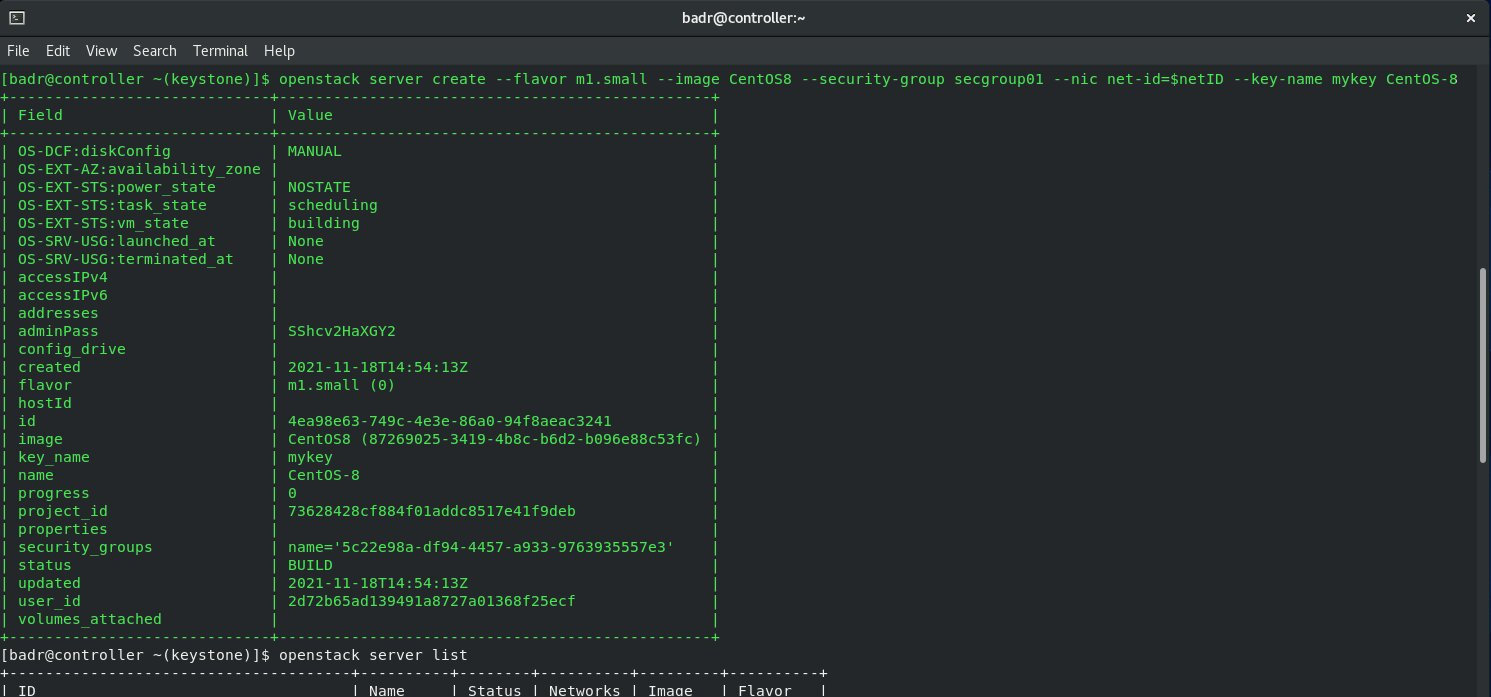
\includegraphics[width=1\linewidth]{Cloud/Creating and Running Instances/create and boot an instance} 
\end{center} 
\caption{create and boot an instance} 
\end{figure} 
\FloatBarrier
\\

\section{Configure security settings}





\par Now let's see the status the Openstack server.
\\
\begin{figure}[!htb] 
\begin{center} 
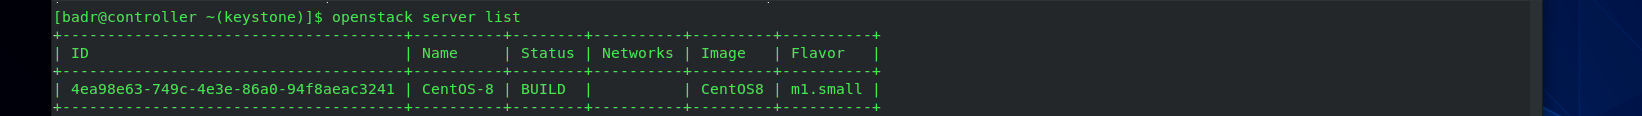
\includegraphics[width=1\linewidth]{Cloud/Creating and Running Instances/show status ([BUILD] status is shown when building instance)} 
\end{center} 
\caption{show status ([BUILD] status is shown when building instance)} 
\end{figure} 
\FloatBarrier
\\


\par Configuration for the security group you created above to access Internet Control Message Protocol.
\\
\begin{figure}[!htb] 
\begin{center} 
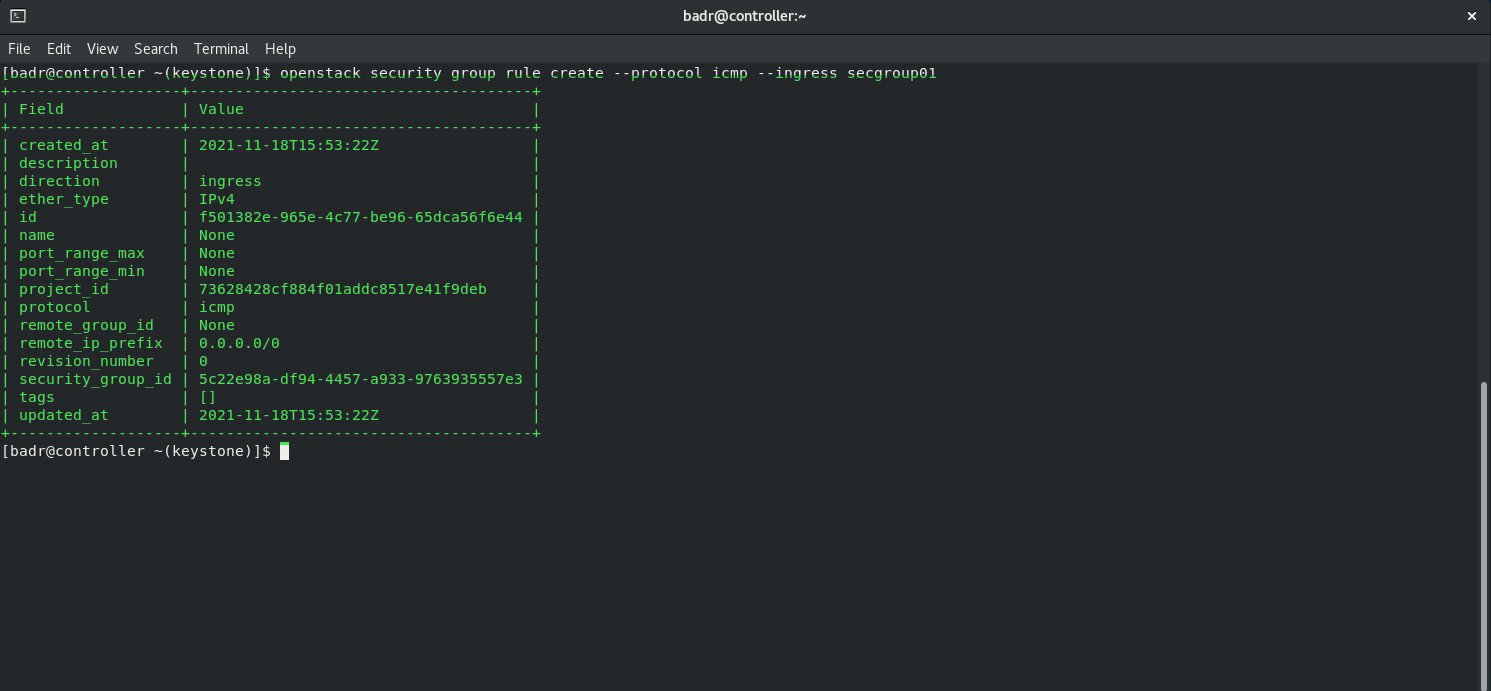
\includegraphics[width=1\linewidth]{Cloud/Creating and Running Instances/permit ICMP} 
\end{center} 
\caption{permit ICMP} 
\end{figure} 
\FloatBarrier
\\
\section{Login to the instance with SSH.}

\par Configuration for the security group you created above to access SSH.
\\
\begin{figure}[!htb] 
\begin{center} 
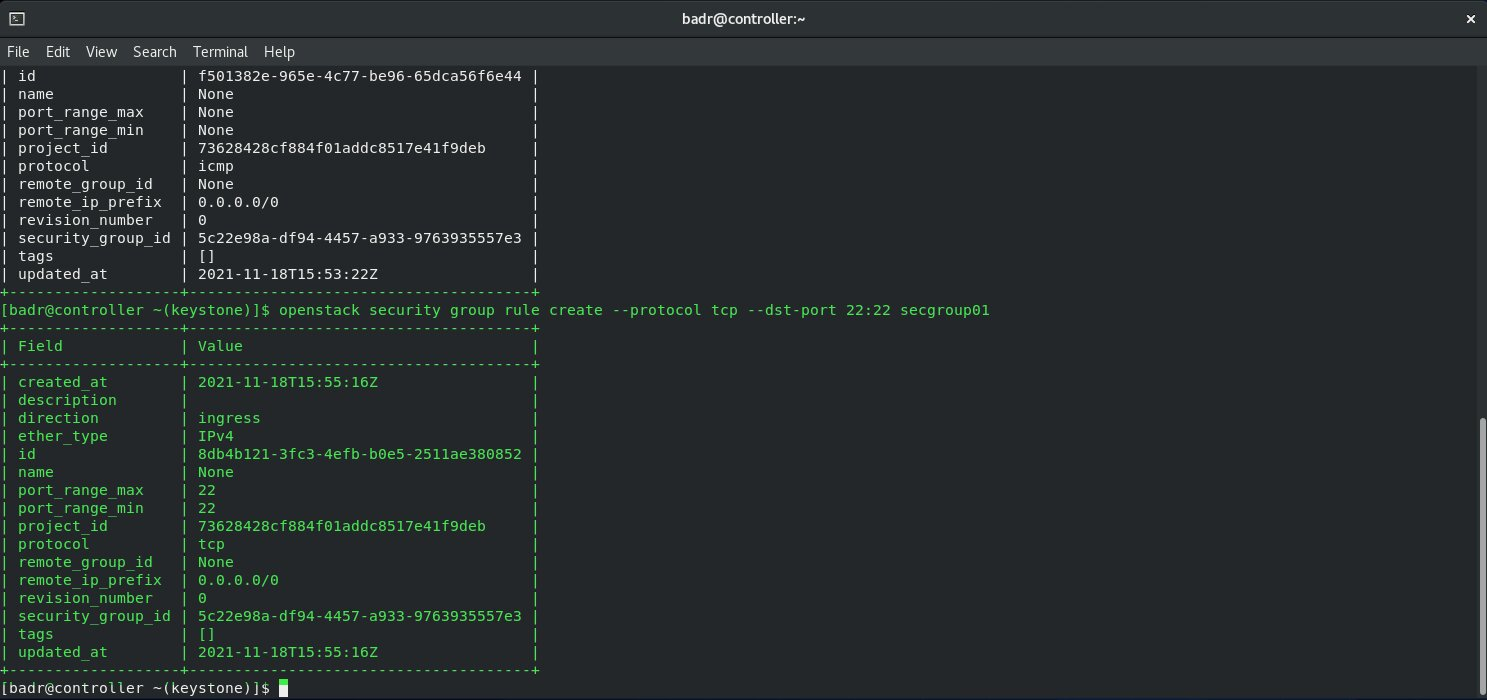
\includegraphics[width=1\linewidth]{Cloud/Creating and Running Instances/permit SSH} 
\end{center} 
\caption{permit SSH} 
\end{figure} 
\FloatBarrier
\\\
\par In this step, we couldn't preform the ping neither the ssh connection, after doing some researches we found that our server is always stuck at the build state, and for the majority in the class it's show an error. but the expected result is shown figure 9.11.
\\
\begin{figure}[!htb] 
\begin{center} 
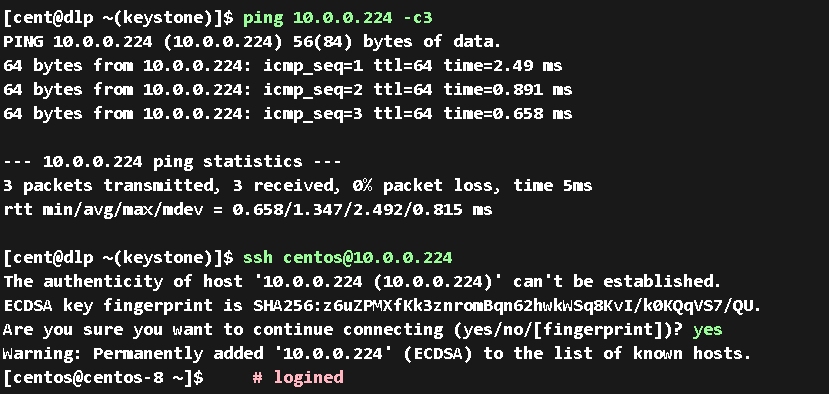
\includegraphics[width=1\linewidth]{Cloud/Creating and Running Instances/C_1_expected_result_for_us_we_stuck_at_build.png} 
\end{center} 
\caption{Ping and connect to the server instance using ssh} 
\end{figure} 
\FloatBarrier
\\
\section{Start or Stop an instance}

\\
\par we couldn't preform theses set of operations on our instance because it's always stuck at the building state. and in this state we cant alter the instance state but the expected results are shown in the figure 9.12
\\
\begin{figure}[!htb] 
\begin{center} 
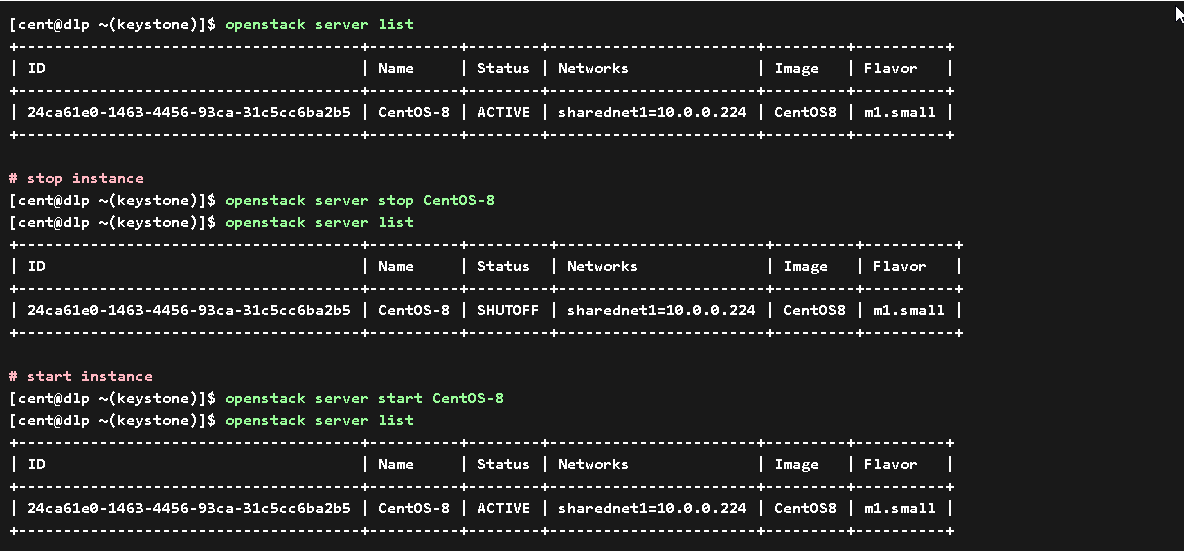
\includegraphics[width=1\linewidth]{Cloud/Creating and Running Instances/C_3_expected_result_since our server us stuck at building process we can't do theses manipulation .png} 
\end{center} 
\caption{Stopping and starting a server instance} 
\end{figure} 
\FloatBarrier
\\

\section{Web Browser to get VNC console.}
\par Now as our server is Active, sometimes we may need to connect to our instance using the typical GUI rather than using a ssh connection. in order to do so we should use the VNC connection protocol, thus in this command we extract the UL that will allow us to connect using the VNC. As our instance is stuck at build status, we couldn't preform theses sets of operation; since a server in the build status can't have an URL for VNC connection, thus the figure 9.13 shows the expected result. 
\\
\begin{figure}[!htb] 
\begin{center} 
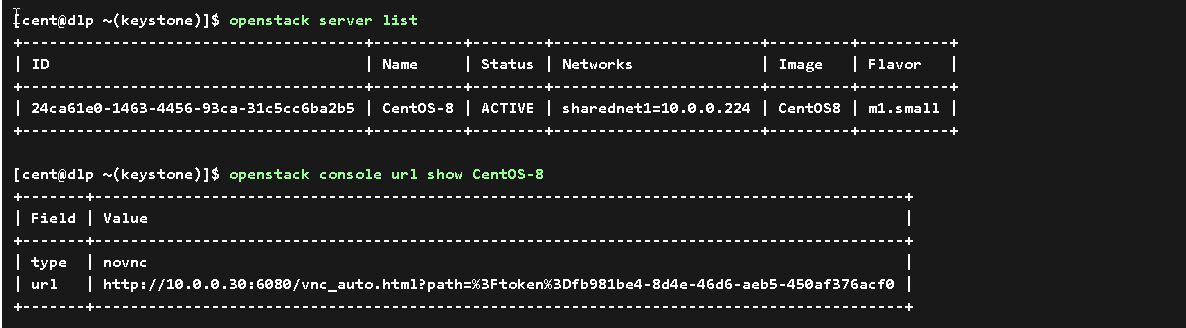
\includegraphics[width=1\linewidth]{Cloud/Creating and Running Instances/C_4_expected_result_since our server us stuck at building process we can't do theses manipulation .png} 
\end{center} 
\caption{getting the URL for VNC conncetion} 
\end{figure} 
\FloatBarrier
\\

\\
\\

\par As our instance is always stuck at the build status we couldn't connect to it using the VNC protocol. But the expected result is shown at the figure 9.14
\begin{figure}[!htb] 
\begin{center} 
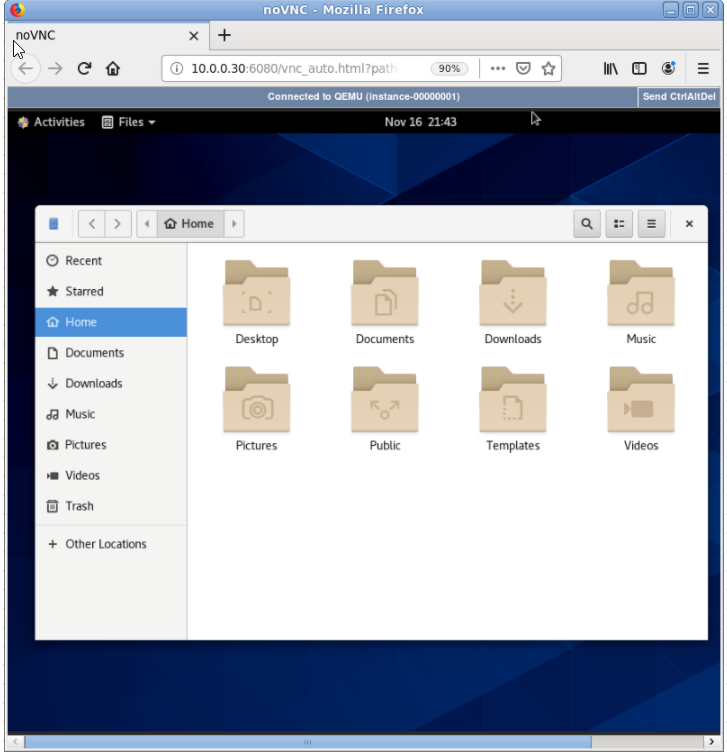
\includegraphics[width=1\linewidth]{Cloud/Creating and Running Instances/C_2_excpected_result_for_us_it_didn't work because of C_1.png} 
\end{center} 
\caption{Connecting to the server instance using VNC console} 
\end{figure} 
\FloatBarrier

\end{spacing}